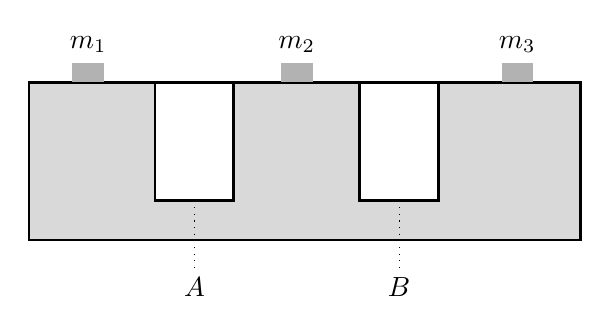
\begin{tikzpicture}
  % filled solid block with two rectangular wells cut out
  \begin{scope}
    \clip (0,0) rectangle (7,2);
    \fill[gray!30] (0,0) rectangle (7,2);
    % wells (white cut-outs) open at top
    \fill[white] (1.6,0.5) rectangle (2.6,2.01);
    \fill[white] (4.2,0.5) rectangle (5.2,2.01);
  \end{scope}
  \draw[line width=1pt] (0,0) rectangle (7,2);
  % well outlines
  \draw[line width=1pt] (1.6,2) -- (1.6,0.5) -- (2.6,0.5) -- (2.6,2);
  \draw[line width=1pt] (4.2,2) -- (4.2,0.5) -- (5.2,0.5) -- (5.2,2);
  % masses on top surface of the columns
  \fill[gray!60] (0.55,2) rectangle (0.95,2.25);   % m1
  \fill[gray!60] (3.2,2) rectangle (3.6,2.25);      % m2
  \fill[gray!60] (6.0,2) rectangle (6.4,2.25);      % m3
  \node[above] at (0.75,2.25) {$m_1$};
  \node[above] at (3.4,2.25) {$m_2$};
  \node[above] at (6.2,2.25) {$m_3$};
  % base points A and B under the wells
  \draw[dotted] (2.1,0.5) -- (2.1,-0.35);
  \draw[dotted] (4.7,0.5) -- (4.7,-0.35);
  \node[below] at (2.1,-0.35) {$A$};
  \node[below] at (4.7,-0.35) {$B$};
\end{tikzpicture}
